Pro hraní hry je potřeba mobilní telefon s aplikací Codeventure, herní kartičky a zobrazovací zařízení, na kterém lze spustit webová aplikace. Nejlepší herní požitek hráč získá při velké ploše zobrazovacího zařízení. Hra běží na doméně: \url{https://www.codeventure.cz/}.\par
Prvním krokem je vytvoření herního účtu, kde se ukládá jednotlivý postup hráče hrou. Následuje stažení mobilní aplikace, kde se hráč přihlásí již vytvořeným účtem. Mobilní aplikaci najdeme v obchodě Goole Play pod názvem Codeventure, \url{https://play.google.com/store/apps/details?id=cz.codeventure.codeventure}.\par
Poté se přesune ve webové aplikaci do hry, kde uvidí první ostrov. Dále hráč využívá pouze mobilní telefon, a to jako ovladač. Na mobilím zařízení si zvolí ostrov a úroveň, kterou chce splnit.\par
Před spuštěním levelu se hráči ukáže slovní zadání úkolu. Dalším krokem je vyobrazení herního zadání ve webové aplikaci a v mobilní spuštění fotoaparátu pro naskenování kartiček. Hráč musí pro úspěšné splnění úrovně seskládat validní a správnou sekvenci kartiček a poté ji naskenovat. Na obr. \ref{fig:pohled-hrace} můžeme vidět herní zadání a naskenovanou karetní sekvenci.\par
Po vyhodnocení se hráči na mobilním telefonu zobrazí, jestli uspěl, či nikoliv. Jednotlivé úrovně může opakovat, nebo může zvolit jinou úroveň. Hra se snaží hráče nabádat k používání sofistikovanějších řešení a díky tomu jej posouvat. 

\begin{figure}[h]
    \centering
    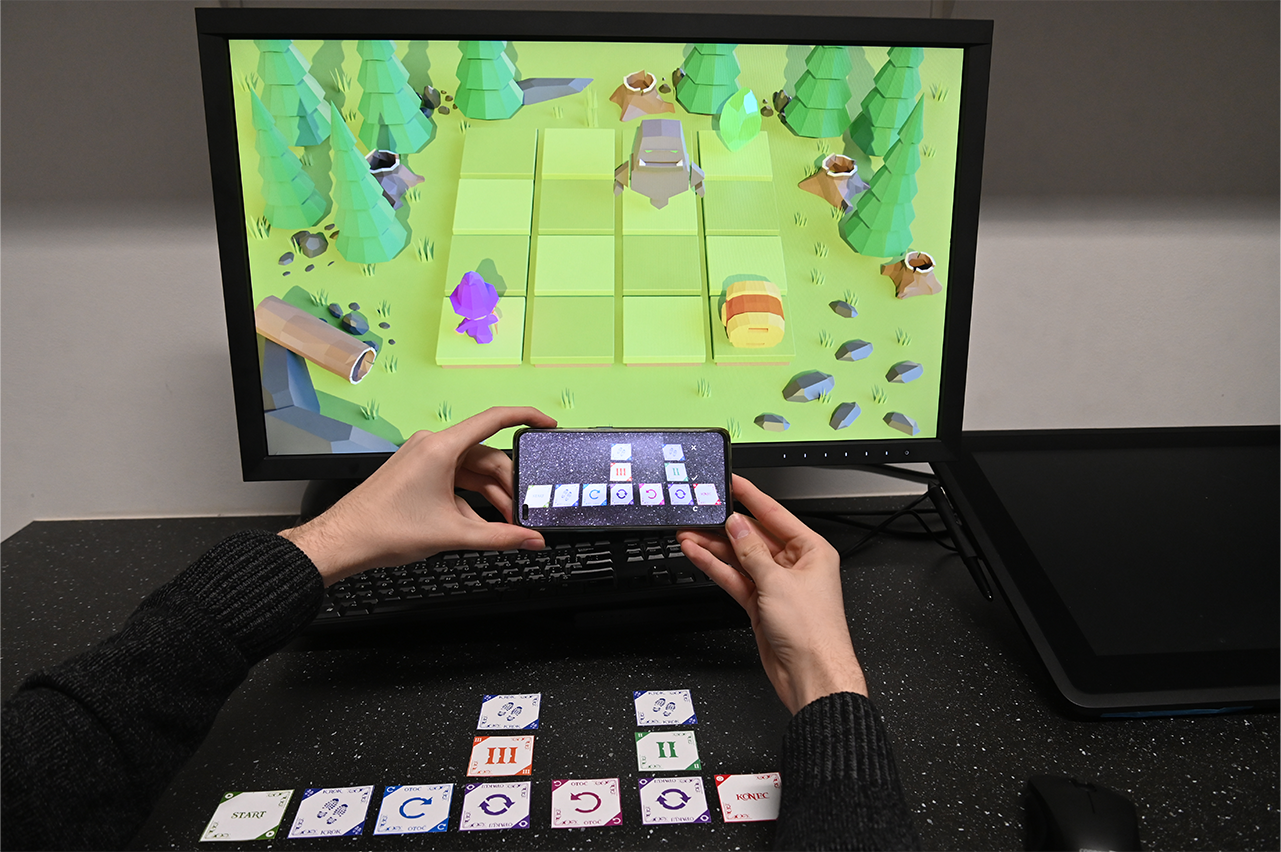
\includegraphics[width=0.6\textwidth]{img/pohled-hrace.png}
    \caption{Pohled hráče.}
    \label{fig:pohled-hrace}
\end{figure}